%!TEX root = da-screen.tex

The defining property of fast distributed algorithms is \emph{locality}: if we run a distributed algorithm for $t$ time steps, then nodes can only be aware of information that is available within distance at most $t$ from them. In this chapter we will see why this is the case, and what consequences it has.

\section{Locality}

Locality is easiest to understand through an example. Consider the following network, familiar from the previous section:
\begin{center}
    \includegraphics[page=\PIntroId]{figs.pdf}
\end{center}
Let us focus on node number $15$. Initially, there is only one node in the network that is aware of the existence of such a node\mydash the node itself. Let us highlight the set of nodes that are aware of node $15$ at time {\boldmath $t = 0$}:
\begin{center}
    \includegraphics[page=\PIntroTA]{figs.pdf}
\end{center}
All other nodes are completely unaware of the existence of node number $15$. For example, for all that they know, we might equally well have the following instance, in which we do not have any node with identifier $15$:
\begin{center}
    \includegraphics[page=\PIntroIdX]{figs.pdf}
\end{center}

Now let us consider what happens at time {\boldmath $t = 1$}, after one communication round. In this round, all nodes can exchange messages with their neighbours, simultaneously in parallel. Nodes can send anything that they know to their neighbours. In particular, node $15$ can inform its neighbours about its existence, so after one round, its neighbours $33$ and $20$ may also be aware of it:
\begin{center}
    \includegraphics[page=\PIntroTB]{figs.pdf}
\end{center}
However, the crucial observation is that only these three nodes can be aware of the existence of node $15$. For example, consider node $27$. Before the first round, this node and its neighbours were unaware of node $15$; hence during the first round node $27$ could not learn anything about node $15$ from any of its neighbours.

By a similar reasoning, at time {\boldmath $t = 2$}, after two communication rounds, the set of nodes that may be aware of node $15$ consists precisely of those nodes that are within distance $t = 2$ from it:
\begin{center}
    \includegraphics[page=\PIntroTC]{figs.pdf}
\end{center}
And at time {\boldmath $t = 3$} this information may have propagated up to distance $t = 3$, but not any further:
\begin{center}
    \includegraphics[page=\PIntroTD]{figs.pdf}
\end{center}
Of course the same reasoning holds for any node, and for any information related to the node. For example, at time $t = 3$, precisely these nodes are aware of the existence of node $13$, and precisely these nodes know that node $13$ is a node of degree $1$, i.e., it has got only one neighbour:
\begin{center}
    \includegraphics[page=\PIntroTDB]{figs.pdf}
\end{center}

Naturally, if a node stops after time $t$, whatever output it produces can only depend on what it knows, and as we have seen, a node can only know information that is available at distance $t$. This is the crux of locality in distributed computing: time and distance are interchangeable; in a \emph{fast} algorithm, nodes have to make decisions based on information that is available \emph{near} them.

\subsection{Simple Consequences of Locality}

FIXME

\subsection{Not So Simple Consequences of Locality}


FIXME: No deterministic symmetry breaking in anonymous networks. Linial's lower bound.

FIXME:

In the previous chapter, we have seen examples of problems that can be solved with a distributed algorithm in the port-numbering model. However, there are many problems that cannot be solved.

As a very simple example, let $N = (V,P,p)$ be a port-numbered network with two nodes, $u$ and $v$, that are connected to each other:
\begin{center}
    \includegraphics[page=\PPnnTwoNode]{figs.pdf}
\end{center}
Assume that we are given a labelling $f(u) = f(v) = 0$. Now let $A$ be any distributed algorithm, and consider the execution of $A$ on $(N,f)$. As the local inputs of $u$ and $v$ are identical, we will have $x_0(u) = x_0(v)$ after the initialisation, that is, nodes $u$ and $v$ have \emph{identical states before round $1$}. It follows that the message sent by $u$ to $v$ in round $1$ is the same as the message sent by $v$ to $u$ in round $1$. Therefore we will have $x_1(u) = x_1(v)$, that is, nodes $u$ and $v$ have \emph{identical states after round $1$}. By induction, we have $x_t(u) = x_t(v)$ for any round $t$. In particular, if $A$ stops in time $T$, we will have $x_T(u) = x_T(v)$, i.e., both $u$ and $v$ produce the same local output.

This reasoning already shows that $A$ cannot produce a proper colouring, a maximal independent set, a minimum vertex cover, etc.\mydash in each of these cases nodes $u$ and $v$ would have to produce distinct outputs. We generalise this observation in Chapter~\ref{ch:covering-map}, when we introduce a very useful graph-theoretic tool, covering maps.

There are also many problems that can be solved with a distributed algorithm, but it requires a lot of time. Techniques that are useful in proving time lower bounds will be introduced in Chapter~\ref{ch:local-neighbourhoods}.
